
\chapter{What falsifies Aryan Invasion Theory (AIT)?}\label{chap08}

\Authorline{Nilesh Nilkanth Oak}


\section*{Abstract}

Aryan invasion theory\index{Aryan invasion theory} was not a theory but a dogma. This is and was the reality of AIT from the time it was conceived in late 18th century CE. While it came out the desire to solve the problem of similarity between European languages and Sanskrit, it developed into a racial theory\index{racial theory} that sought to differentiate not only Europeans from Indians, but also claim racial differences within Indian population. The dogmatic character of AIT can be understood if it is tested against the basic framework of scientific method. The four key elements of AIT are outlined and employed it build specific testable statements, if objectively validated, would falsify AIT.

The paper mentions contributions of researchers from linguistics and archaeology that falsifies AIT and then decisively falsifies AIT, with the original work of author from astronomy combined with evidence from varied fields of hydrology, geology, geophysics, climatology, oceanography, climatology, relative chronology of Ṛgveda and genealogies of kings and sages of Ṛgveda and Mahābhārata and Rāmāyaņa.

The falsification of AIT and its comprehension by Indic population is critical in its fight against ‘breaking India’ forces. AIT is falsified; however, there is a need to communicate these findings in a language lay people can comprehend and communicate to others.


\section*{1. Pūrvapakṣa\index{Purvapaksa@Pūrvapakṣa} - Aryan Invasion Theory (AIT)}

While there are numerous individuals who will employ the word AIT, very few are willing to explain what it is. This hesitation is due to good reasons. AIT is based on lot of conjectures but with zero evidence. In fact, all newfound evidence has forced the believers of AIT to modify it into Aryan Migration theory\index{Aryan Migration theory} (AMT) or Indo-Aryan Migration theory.

\subsection*{1.1 Theories are proposed to solve problems}

What was the problem AIT trying to solve?

Dr. Shiv Shastry writes (2017a)

\begin{myquote}
When European scholars came to India along with the British, they were surprised to discover the similarity between Sanskrit and European languages like Latin, French, German and English. Even more significant was the discovery by Europeans of Sanskrit grammar. Until then, European linguists knew that their own languages in Europe were somewhat similar, but it was the revelation of Sanskrit grammar that made them aware of how and why European languages were related.
\end{myquote}

Beginning with this desire to solve the problem of similarity between European languages and Sanskrit, how AIT turned into a racist theory which in turn added ‘breaking India’ elements by speculating Aryan vs Dravidian races within India is a story by itself. How this conjecture of AIT became a mainstream theory in Indology studies, despite characteristic lack of any evidence is also a story worth recollecting. Fortunately, Dr. Shiv Shastry (2017a, 2017b) narrates these developments well. Having said that, a criticism of a theory should focus on the methods and the results of examining it logically and not how various assertions of a theory were conceived.

It is possible to enumerate the steps used to test a scientific theory.

\begin{enumerate}[{\rm 1)}]
\itemsep=0pt
\item Logical comparison of the conclusions, of a theory, among themselves. This allows testing of internal consistency of a theory.

 \newpage

 \item Investigation of the logical form of the theory. This allows to examine whether the theory has the character of an empirical or scientific theory, or whether it is, purely tautological.

 \item This step would include comparison to the theory with other theories to determine if the theory would constitute a scientific advance, assuming it survives various other tests.

 \item Testing of the theory by making predictions based on it and then comparing them against the actual evidence.

\end{enumerate}

Unfortunately, AIT is formulated and is discussed, by its proponents, in a non-scientific fashion and thus, the testing of it via these four steps becomes impossible. This can be illustrated with the logic of scientific method. For example, a specific theory leads to various predictions and one of the predictions includes the solution to the problem it is intended to solve.


\subsection*{1.2 AIT as dogma}

Let’s evaluate AIT in the context of five elements of scientific method described in Figure 1.

\begin{figure}[!htbp]
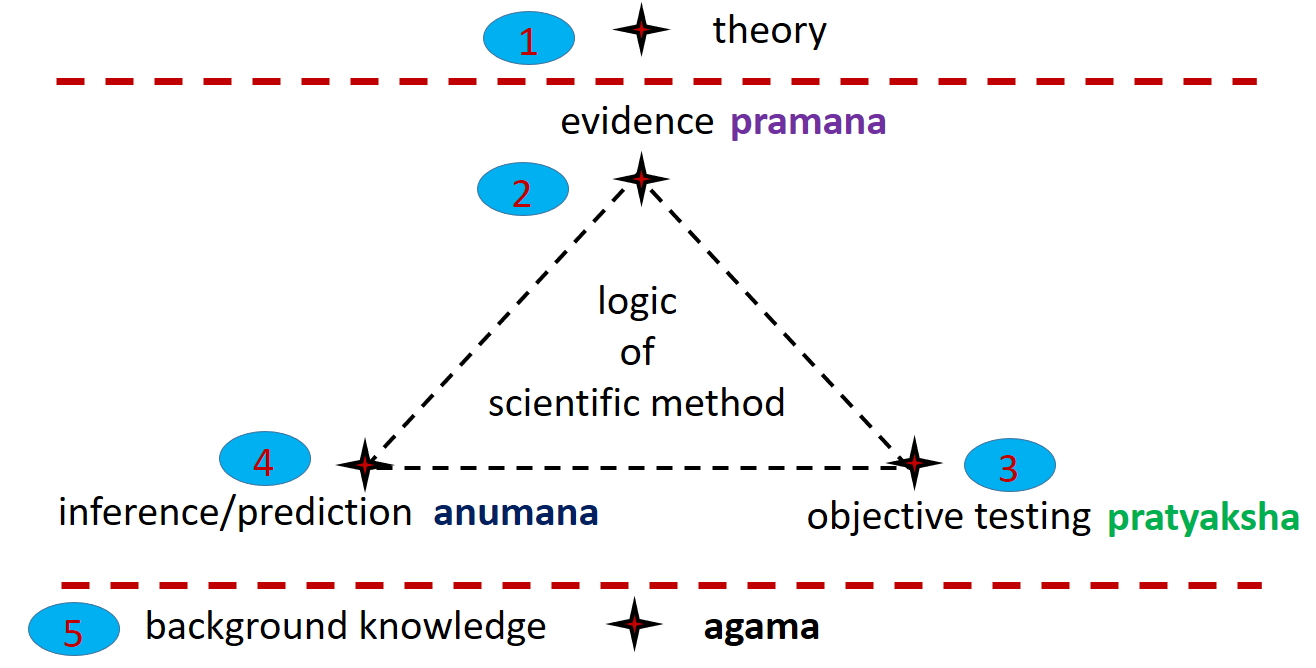
\includegraphics[scale=0.2]{images/8-01.jpg}
\caption{}\label{art8-fig01}
\end{figure}

\begin{enumerate}[{\rm 1)}]
\itemsep=0pt
\item The people who called themselves ‘Āryan’ came from some unknown location ‘outside India’ into ‘the greater India’ sometime between 2000 BCE and 1500 BCE, and they brought the Sanskrit language or a precursor to Sanskrit language.

 While this is taken as the statement of Aryan invasion theory, it does not fit the criteria of what is expected of a scientific theory. The statement of a scientific theory is expected to be general in nature in the context of its background assumptions that allows multiple predictions. For example, the general theory could have been stated as ‘people do migrate from one geographical region to another and when they do it, they tend to take their language, culture, belief systems, science and technology along with them’. No such thought had gone into formulating the statement of ‘Aryan invasion’ theory or assuming such background assumptions, rather the evolution of background assumptions as well as additional predictions was an afterthought.

 \item What a scientific theory would consider an explanation of a phenomenon, i.e. one of the consequences (predictions) of the theory, i.e. the solution to the problem the theory was designed to solve, was the core statement of the theory itself. We would repeat the statement in (1) as the desired element of scientific method, expected in (2). The explanation (pramāņa) is that the similarity between European languages and Sanskrit can be explained due to this fact of ‘Aryans’ bringing either Sanskrit or precursor to Sanskrit to greater India\index{greater India}.

 \item This corner of ‘pratyakṣa’, of the pratyakṣa-anumāna-pramāņa triangle must remain empty, since there was nothing to test objectively and nothing was tested.

 \item This corner of ‘anumāna’, of the pratyakṣa-anumāna-pramāņa triangle must also remain empty, since all the inferences (four features underlined in (1)) were assumed in the formulation of the statement of theory (1) and its explanation (2).

 \item As explained in (1), various background assumptions viz. Aryans as a race, elements of horses, chariots, features attributed to Aryans, location of their origin were simply inserted as afterthoughts.

\end{enumerate}

The lack of scientific logic in the formulation of AIT is the reason why it should be understood as a dogma and not a scientific theory. AIT or AMT should be termed as Aryan invasion dogma\index{Aryan invasion dogma} (AID) or Aryan migration dogma (AMD).


\subsection*{1.3 Features of AIT}

While the theory does not make new predictions, the formulation of the theory has placed constraints on various features of the theory. This paper discusses four specific features of AIT and constraints imposed on them. These constraints will be used to decisively falsify AIT. The first two features of AIT include the location and the timing of this claimed invasion as shown in Figure 2.

\begin{figure}[!htbp]
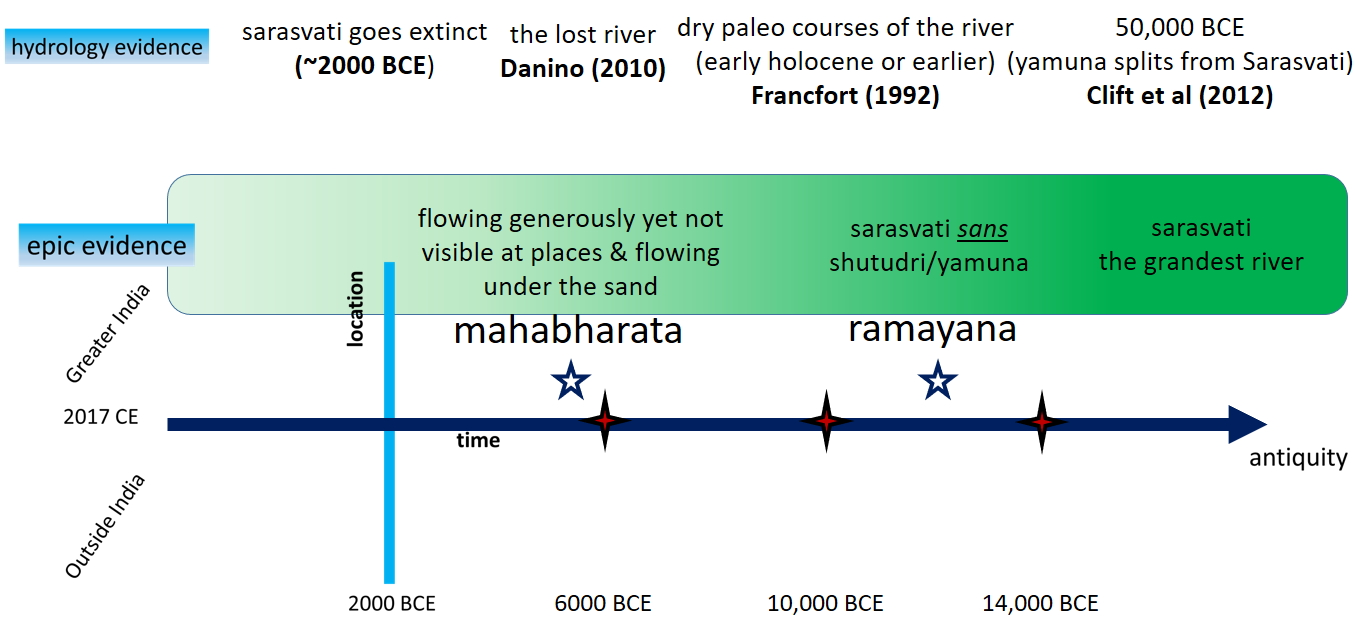
\includegraphics[scale=0.25]{images/8-02.jpg}
\caption{}\label{art8-fig02}
\end{figure}

The vertical axis of location passes through the point of 2000 BCE on the horizontal time axis. This is indeed the upper constraint on the timing of AIT. Notice that time axis begins with our times on the left and goes backward in time to infinity. All AIT proponents agree that the so called ‘Aryan’ invaders came from ‘outside India’ into ‘greater India’, however, there is total disagreement when it comes to fixing the location within ‘outside India’ from where these so called ‘Aryan’ arrived into ‘greater India’.

The greater India, for this paper, is defined as approximate geographical area that constitutes modern countries of Iran, Afghanistan, Pakistan, India, Nepal, Sri Lanka, Bhutan, Bangladesh, Burma \& Thailand. It is also possible to visualize ‘greater India’ with parts of Turkmenistan, Uzbekistan, Tajikistan, Laos, Cambodia \& Indonesia, in addition to all countries mentioned in the previous list. All the countries mentioned in the context of ‘greater India’ are shown in Figure 3.

\begin{figure}[!htbp]
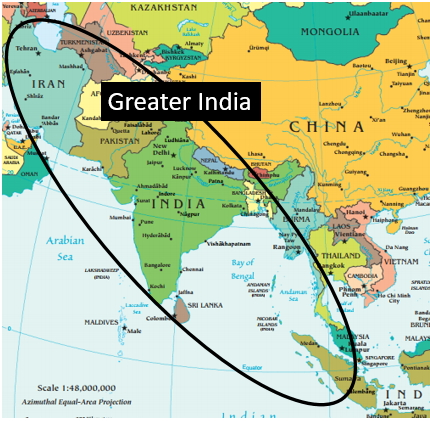
\includegraphics[scale=0.38]{images/8-03.jpg}
\caption{}\label{art8-fig03}
\end{figure}

The additional two features came into India, per AIT theory, when people who called themselves ‘Aryan’ came from somewhere ‘outside India’ into ‘greater India’\index{greater India} sometime between 2000 BCE and 1500 BCE. These ‘Aryans’ brought with them, per AIT theory, Sanskrit language or the precursor to Sanskrit language. The four features of AIT theory can be summarized as follows:

The people who called themselves ‘\textbf{Aryan}’ came \textbf{from some unknown location ‘outside India’ into ‘the greater India’} sometime \textbf{between 2000 BCE and 1500 BCE, and they brought the Sanskrit language or a precursor to Sanskrit language}. These four features of AIT along with their constraints are summarized in Figure 4.

\begin{figure}[!htbp]
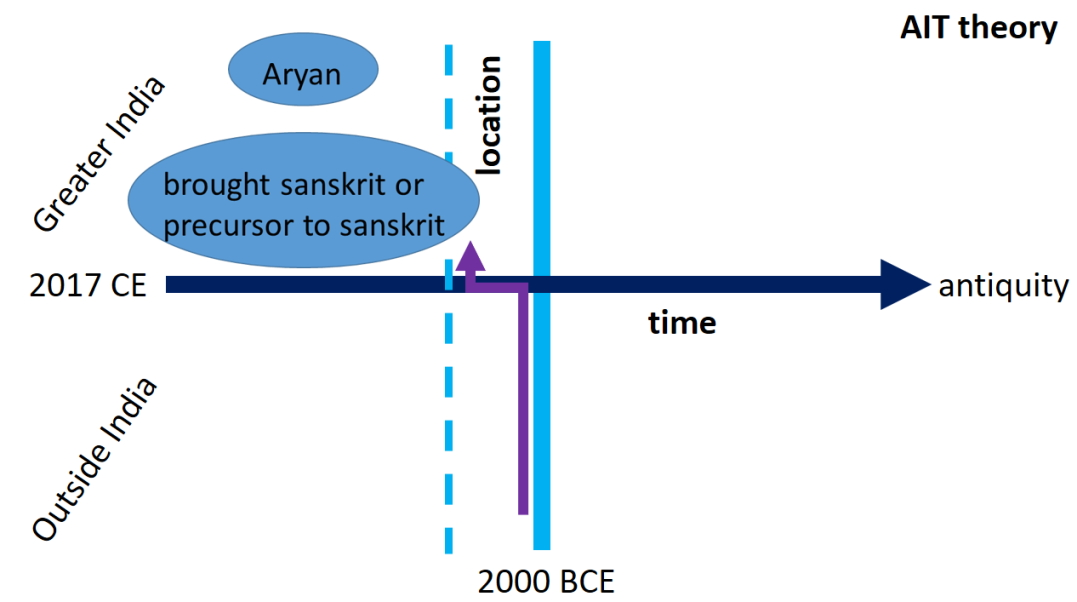
\includegraphics[scale=0.21]{images/8-04.jpg}
\caption{}\label{art8-fig04}
\end{figure}


\subsection*{1.4 Rationale for constraints on AIT}

There is no specific rationale as to why Sanskrit language or precursor to Sanskrit language must have its origin outside India. It is just that AIT proponents are vehement in their claim that the origin of Sanskrit language or its precursor is to found outside India. The same absence of logic or rationale exists when it comes to the so called ‘āryan’ race. AIT proponents have specified constraints on the timing of AIT, both upper and lower limits. These constraints vary from 1000 BCE to 2000 BCE and they are all based on fancy linguistics arguments.


\section*{2 Uttarapakṣa\index{Uttarapaksa@Uttarapakṣa} - Aryan Invasion Theory (AIT)}

Since dogma of Aryan invasion does not result in clear statements for five elements of the scientific method, this paper would focus on four specific feature and corresponding constraints - geographical, linguistic, denominational and chronological – to falsify AIT.

Thus, AIT would be considered falsified if,

\begin{enumerate}[{\rm 1)}]
\itemsep=0pt
\item It can be shown that there is no evidence for ‘Aryan’ anywhere in the world, of course, prior to formulation of AIT

 \item It can be shown that ‘Sanskrit’ language or ‘precursor to Sanskrit language existed in India, long before 2000 BCE

 \item It can be shown that the word ‘Aryan’ itself was a confused derivation of a similar word that existed in India, long before 2000 BCE

 \item It can be shown that Ṛgveda – the oldest available text of humanity, existed in India, long before 2000 BCE

 \item It can be shown that ‘Sanskrit’ language based culture existed in India, long before 2000 BCE

\end{enumerate}


\subsection*{2.1 Let’s kill ‘Aryan’ of Aryan invasion theory}

The so called Aryan invasion theory was formulated, at least first version of it, sometime at the end of 18th century CE. The word ‘Aryan’ is not found inside ‘greater India’ or outside India any time before 18th century CE leading all the way to 2000 BCE, supposedly the upper limit on the timing of AIT. The word ‘Aryan’ is not found inside ‘greater India’ or outside India any time before 2000 BCE, either.


\subsection*{2.2 Researches in Linguistics}

AIT was formulated to solve the problem of similarity between European languages and Sanskrit. This theory should have been put to test by asking question such as ‘if language (Sanskrit or precursor to Sanskrit) was brought by some people from point A to point B, what is the evidence that the language existed at point A?’. The dogmatic proponents of AIT see no need for such rational questions and seeking for their answers. Of course, the problems of AIT run deeper than the question of location and evidence for existence of a specific language (or its precursor) at a specific location. The upper constraint of ~1500 BCE on the timing of AIT is very much due to the necessity of language existence outside India (but its absence within India), before 1500 BCE.

In words of Talageri\index{Talageri, Srikant} (2008:162):

\begin{myquote}
The AIT is built up on a number of extra-Indian factors, which necessarily require that the Vedic Aryans should be brought into India \textit{no earlier than 1500 BCE}.
\end{myquote}

and Talageri (2008:163):

\begin{myquote}
The linguistic case \textit{for the AIT} consists almost entirely of circular arguments and invasionist dogmas.
\end{myquote}

The entire discipline of linguistics, - philology and ‘historical linguistics’ were built on dogmatic principles.

In a series of books published over 15 years, Shri Shrikant Talageri\index{Shrikant Talageri} (1993, 2000, 2008) demonstrated, by employing the same techniques of AIT proponents, that language flow, if at all it occurred, occurred in the opposite direction to what is claimed by AIT proponents and is shown in Figure 5.

Talageri (2008:224) summarizes the entire linguistic argument of AIT:

\begin{myquote}
Therefore, to sum up, there is no linguistic case at all, worth the name, against the OIT case presented by us in our earlier books, and presented again with much more detail in this present book, especially in this chapter. The Indian homeland case presented by us answers all the linguistic requirements perfectly, while the AIT completely fails to answer any of them.
\end{myquote}

Naturally, AIT proponents have become silent on ‘linguistics’.

\begin{figure}[!htbp]
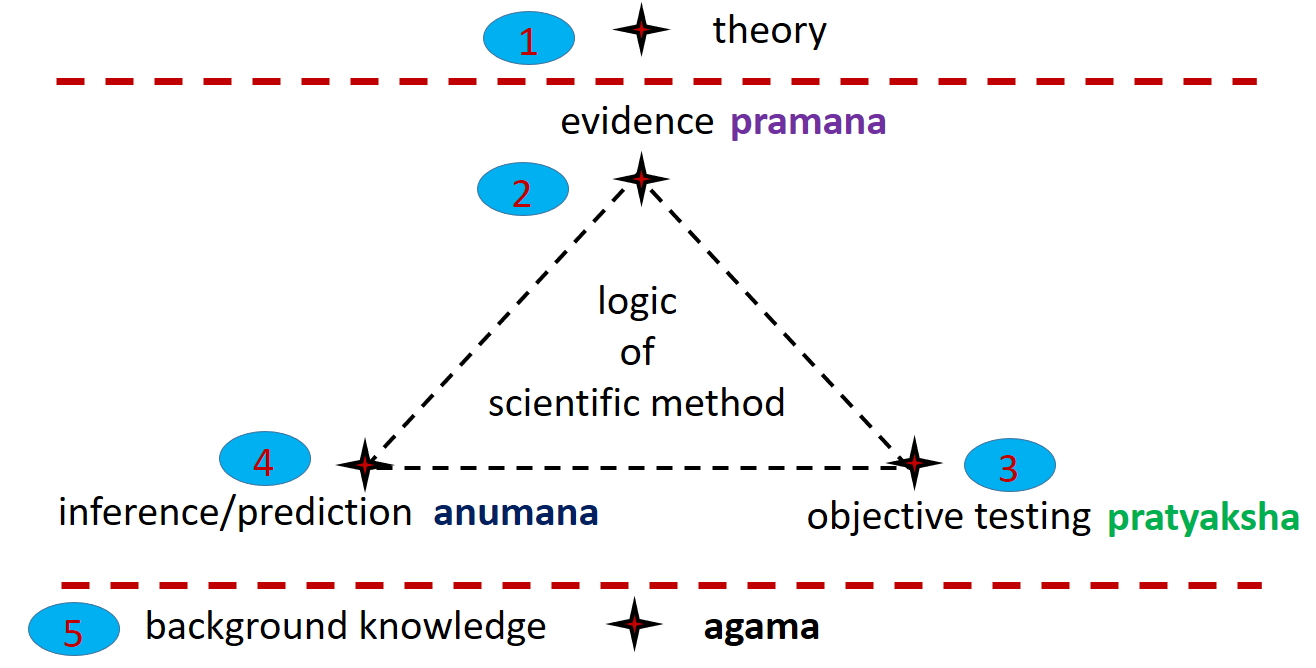
\includegraphics[scale=0.15]{images/8-05.jpg}
\caption{}\label{art8-fig05}
\end{figure}


\subsection*{2.3 Researches in Archaeology}

Talageri (2008:225) writes:

\begin{myquote}
From the very beginning, i.e. from the first moment that the academic search for the Indo-European homeland began, there have been three broad academic disciplines involved in this field of study: linguistics, textual analysis, and archaeology.
\end{myquote}

Enormous research, in the context of Sindhu-Sarasvati civilization\index{Sindhu-Sarasvati civilization} has taken place over the last few decades and inferences from these studies have decisively falsified whatever stray arguments put forth in buttressing the dogma of AIT. Lal (2002, 2009) shows, with the help of archaeology evidence, that continuous civilization existed in India, in the areas of Sindhu and, now extinct, Sarasvati rivers\index{Sarasvati river} for over a period of at least last 9000 years and is represented in Figure 6.

Not surprisingly, AIT proponents have also become silent about archaeology evidence.

\begin{figure}[!htbp]
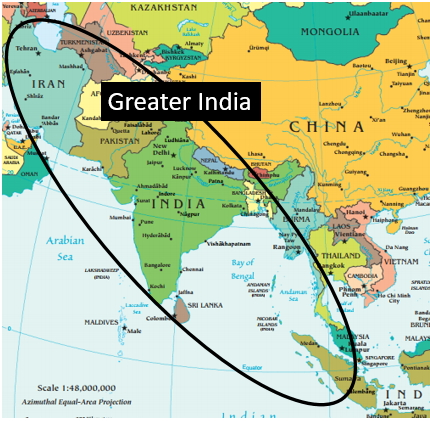
\includegraphics[scale=0.22]{images/8-06.jpg}
\caption{}\label{art8-fig06}
\end{figure}


\subsection*{2.4 Researches in Genetics}

Having lost the fight in the areas of linguistics and archaeology, AIT proponents are clinging to ‘genetics’ with the same hope as a drowning man clutches at the straws. It is reasonable to expect lot more justifications for AIT by AIT proponents in the garb of genetics and hence ‘scientific sounding’ inferences. Such claims would increase in numbers as the science of genetics progresses. Let’s understand why this is already happening and why it would only become more intense with the advances in science and technology of genetics research\index{genetics research}.

Existing genetics research shows that there were migrations in and out of greater India over the period of last 100,000 years. The first detectable migration(s), based on genetics evidence, into greater India possibly occurred 80 to 100 thousand years ago from Africa. There is impressive genetics evidence for multiple migrations, out of greater India to rest of the world over last 80 thousand years. India has also seen migrations from outside India in the last two thousand years. These recent migrations are documents in historical records and can also be validated with the help of genetics. The most common scenario is that of the migration of human beings out of India, post 80 thousand years ago, into rest of the world and is represented in Figure 7.

\begin{figure}[!htbp]
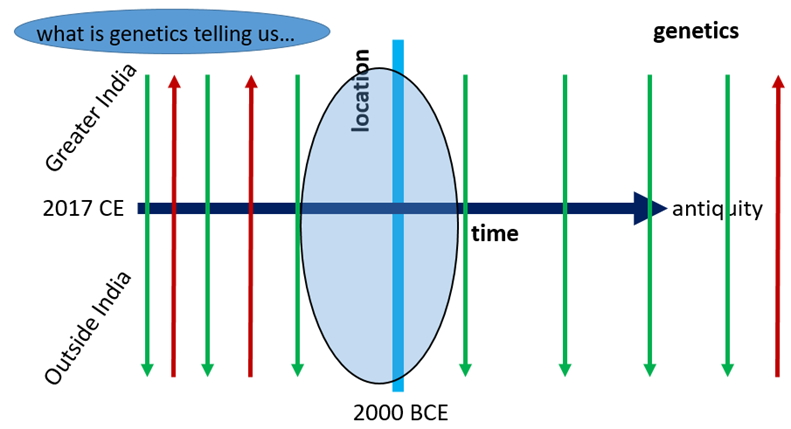
\includegraphics[scale=0.25]{images/8-07.jpg}
\caption{}\label{art8-fig07}
\end{figure}

Red lines represent migration into greater India and green lines represent migration from greater into to the rest of the world. The time interval from 2500 BCE through 1000 BCE is highlighted by an oval and shows no migrations, in or out of India. This is because no reliable data exists for desired level of resolution for this time interval. This is the time interval claimed by AIT proponents for the timing of AIT. We will revisit this time interval soon.

Genetics is capable of detecting direction of gene flow, both on maternal side of the gene (matrilineal) and on paternal side of the gene (patrilineal). The summary research of matrilineal gene tells us that predominantly there was an outflow of ‘mother’ gene from India, after its initial introduction in India some 80 thousand years ago, into rest of the world and is represented in Figure 8 (Metspalu, 2004).

\begin{figure}[!htbp]
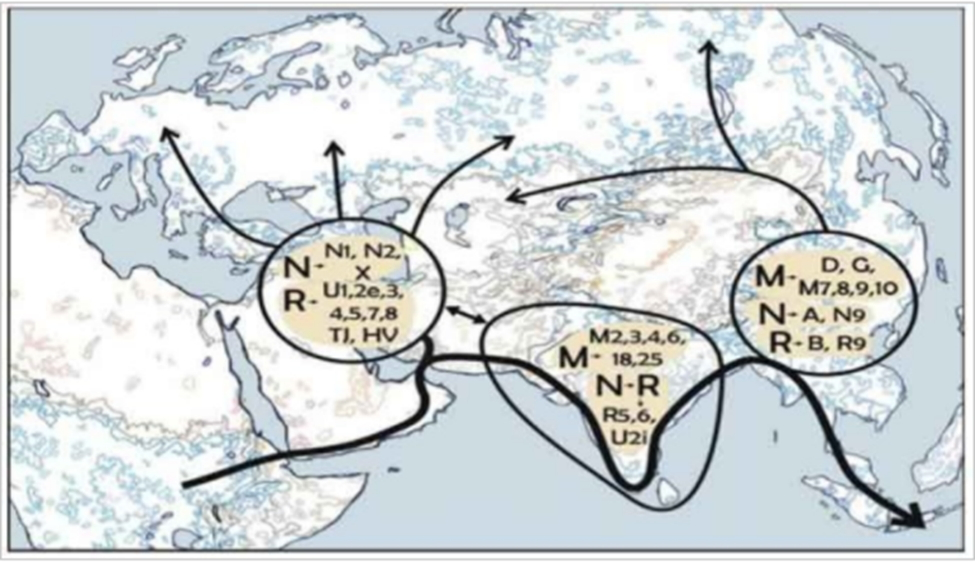
\includegraphics[scale=0.26]{images/8-08.jpg}
\caption{}\label{art8-fig08}
\end{figure}

The patrilineal gene tells the identical story. After its initial introduction in India some 80 thousand years ago, predominant story of patrilineal gene shows evidence of its going out of India, through multiple outward migrations, into rest of the world and is represented in Figure 9.

\begin{figure}[!htbp]
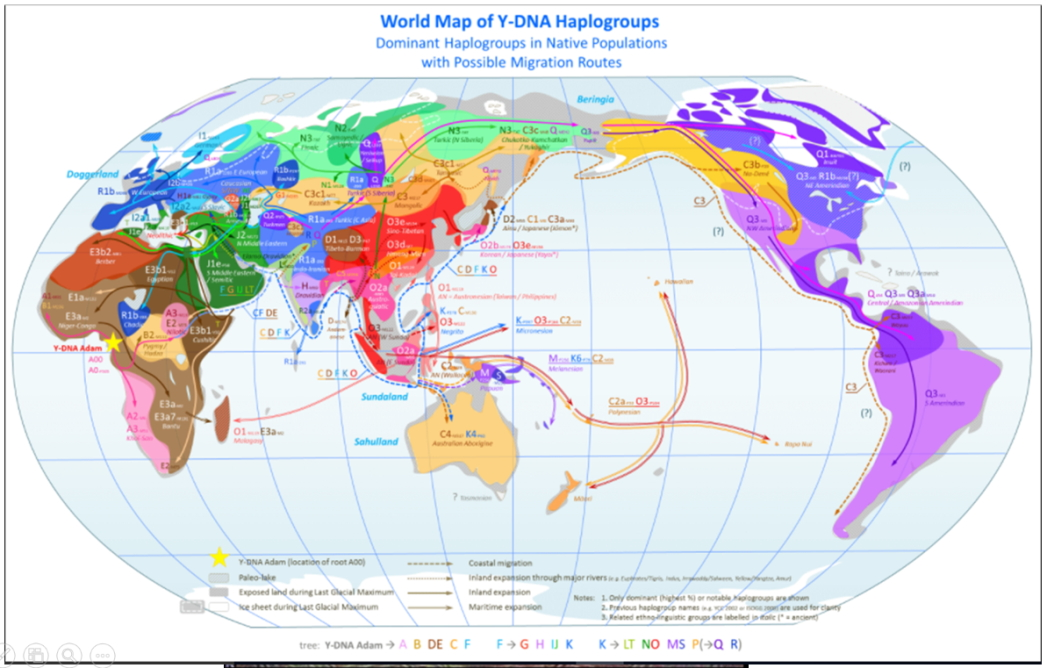
\includegraphics[scale=0.22]{images/8-09.jpg}
\caption{}\label{art8-fig09}
\end{figure}

It is indeed worthwhile to study spread of patrilineal gene from greater Indian homeland into rest of the world and is pictorially represented in Figure 10.

\newpage

\begin{figure}[!htbp]
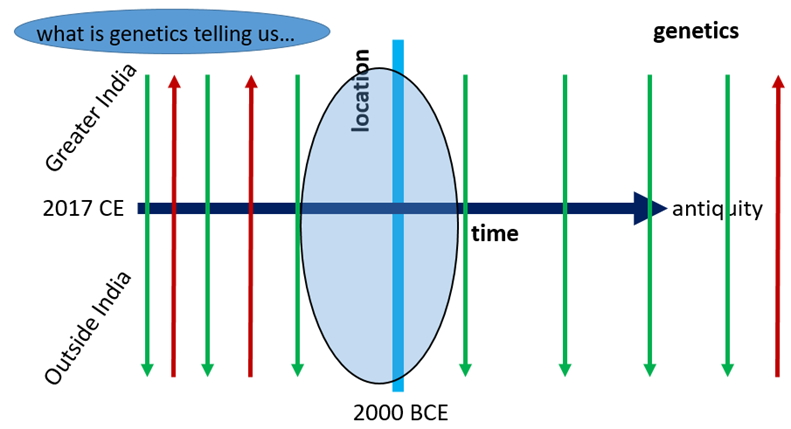
\includegraphics[scale=0.21]{images/8-10.jpg}
\caption{}\label{art8-fig10}
\end{figure}

While this outward gene flow of matrilineal or patrilineal genes may not tell us if their status as migrants was that of nomads or hunter-gatherers, pastoralists or agriculture settlers, the outward gene flow of domestic mouse provides us with evidence to assert that some of these outward migrations carried with them agriculture and civilization. The outward gene flow of domestic mouse, going back to a period of 20 to 30 thousand years ago, provides a critical evidence in constructing the picture of ancient migrations, and is represented in Figure 11 (Bonhomme, 2007).

\begin{figure}[!htbp]
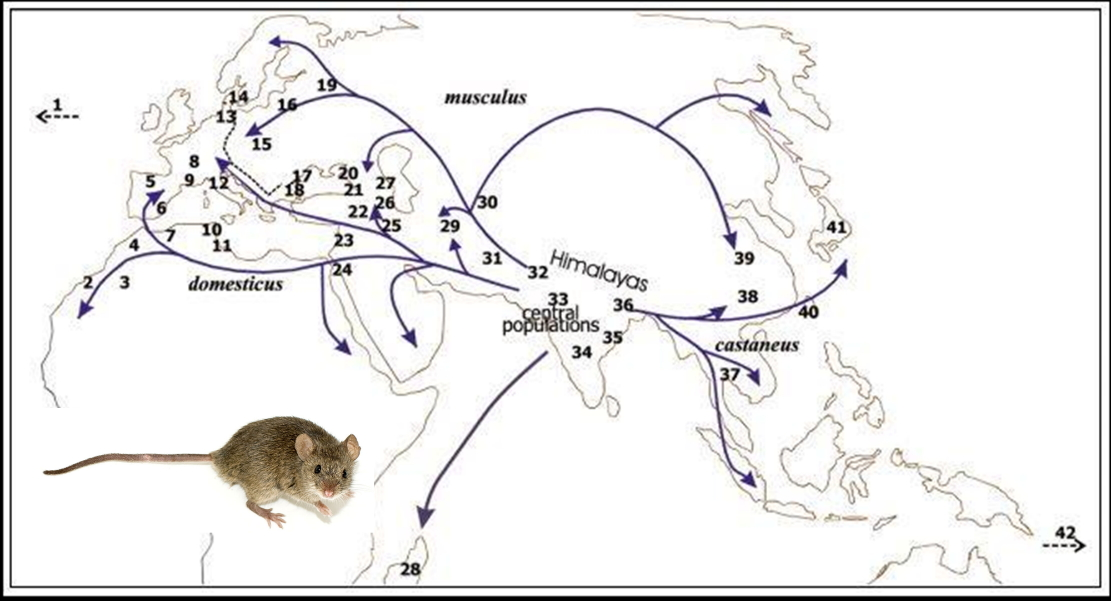
\includegraphics[scale=0.22]{images/8-11.jpg}
\caption{}\label{art8-fig11}
\end{figure}

\newpage

It is well to keep in mind that none of this would deter AIT proponents who are wedded to dogma of someone brining Sanskrit or precursor to Sanskrit, from somewhere outside India, into greater India. And for this very reason, it is also important to understand the limitations of three disciplines of studies discussed so far: linguistics, archaeology \& genetics.


\subsection*{2.5 Limitations of linguistics, archaeology \& genetics}

It is not possible to set chronology to changes in languages and existing attempts are at best crude approximations. Genes don’t carry known markers of languages and archaeology has to do its own guesswork regarding the culture and the language in the absence of epigraphic evidence.

To comprehend limitations of these three disciplines of studies, in the context of AIT, it is useful to analyze what happens when evidence from two of these three disciplines is combined. For example, archaeology evidence is incapable of telling us about the language(s) spoken by a specific civilization and at specific time, unless we have epigraphic evidence\index{epigraphic evidence} and we can decipher what is written in such evidence. As of now, we do not have any epigraphic archaeological evidence in India that is been convincingly deciphered and can be dated to beyond 500 BCE.

\newpage

Genes don’t encode the language information however this scientific principle is being ignored in majority of genetics studies, especially in the context of India and those who claim to draw inferences about AIT, based on genetics evidence. In fact, combining genetics evidence with dogmatic conjectures of AIT has become a pastime of many and playground of great many imposters.

Archaeology\index{Archaeology} can interact with genetics\index{genetics} when human skeletons are found in archaeological excavations and if their DNA (ancient DNA) can be extracted. Recently human skeletons were found at certain excavations in Sindhu-Sarasvati civilization\index{Sindhu-Sarasvati civilization} and results from tests of ancient DNA are awaited. Let’s imagine two possible scenarios for this outcome. Suppose the DNA identified with well-known haplogropus already identified on Indian subcontinent, it will turn out to be no news. On the other hand, if the DNA identified happens to match with one of the youngest branch of, say R1a (haplogroup) which is also present in Europe and central Asia, all hell will break loose, and expect AIT proponents to flood the social media and peers reviewed journals touting such an occurrence as evidence of AIT. On the other hand, a serious researcher of genetics would not be surprised by such a finding. After all, there is evidence of people migration in and out of India over thousands of years and as science of genetics progresses and as resolution improves, one should indeed expect to detect additional migration instances, both, in and out of greater India, for various timelines and that would also fall between the claimed interval of 2000 BCE –1500 BCE by AIT proponents.


\subsection*{2.6 Scientific Poison Pills\index{Scientific Poison Pills} (SPP)}

Linguistics work of Shri Talageri and archaeology findings of Sindhu-Sararsvati region have decisively falsified AIT. The reaction of AIT proponents have been to ignore the work of Shri Talageri on linguistics and to minimize the claimed importance of archaeology evidence (by these very proponents of AIT) for the survival of AIT and to hope that younger haplogroups\index{haplogroups} show up in ancient DNA of Indian archaeology samples, for specific time intervals claimed by AIT, whose parent gene is already present in either Europe or central Asia shows up in ancient DNA on Indian soil.

\newpage

Numerous new developments have taken place in the context of chronology of Indian history. Majority of these chronology markers are based on empirical and objectively testable evidence where inferences are drawn with deductive logic and thus have withstood some of the toughest demands expected of a scientific theory, testing and inferences. Each one of them act as deadly poison pill for AIT. In the remainder of the paper we will enumerate few poison pills.

\subsubsection*{2.6.1 Astronomy evidence from the epics (Mahābhārata \& Rāmāyaņa)}

There are more than 130 claims for the chronology of Mahābhārata war\index{Mahabharata war@Mahābhārata war} and more than 15 claims for the chronology\index{chronology} of Rāmāyaņa. Unfortunately, majority of them are plagued with poor comprehension of evidence or total ignorance of the logic of scientific method.

Oak (2011) revolutionized the chronology research of Mahābhārata by demonstrating for the first time an objectively testable solution to the problem of Arundhatī Vasiṣṭha\index{Arundhati Vasistha@Arundhatī Vasiṣṭha} (AV) observation. This lead to a well-defined interval of about 6500 years (11091 BCE – 4508 BCE) for the year of Mahābhārata war. This discovery led to the prediction for the duration of Bhishma\index{Bhishma} on the bed of arrows to be equal to 98 days. What is fascinating is that further investigation of Mahābhārata evidence showed that the text indeed has evidence for duration of Bhishma on the bed of arrows to be more than 92/95 days. This discovery in turn led to next prediction of the lunar month of the war to be that of Mārgaśīrṣa\index{Margasirsa@Mārgaśīrṣa} and the timing of the war to be that of early Śarad season. Again, the evidence from the pages of Mahābhārata text showed that the war indeed took place during the lunar month of Mārgaśīrṣa and that the timing of the war was that of the early part of Śarad season. Total of more than 200 astronomy and chronology evidence of Mahābhārata\index{Mahabharata@Mahābhārata} text was tested in this prediction-testing-validation pattern to arrive at 5561 BCE as the year of Mahābhārata war.

Oak (2014) employed identical methodology in determining chronology of Rāmāyaņa. Four independent astronomy observations from four different kāņḍa of Vālmīki Rāmāyaņa and their objective testing led to the prediction of broad time interval [10,000 BCE – 17500 BCE] for the plausible timing of Rāmāyaņa\index{Rāmāyaņa@Rāmāyaņa}. Unique evidence of comet near nakṣatra Mūla led to a conjecture for the year of Rāma-Rāvaņayuddha, within this time interval, which in turn was corroborated by more than 300 astronomy and chronology observations of Vālmīki Rāmāyaņa. The chronology for 30-year period of Rama’s life thus obtained led to various predictions of seasons for the specific events of Rāmāyaņa. More than 200 additional descriptions of seasons from Vālmīki Rāmāyaņa provided corroboration for these predictions. Thus, more than 500 specific observations and their objective testing led to 12209 BCE as the year of Rāma-Rāvaņayuddha.

No one should accept above claims at a face value and all curious individuals should test them, each one of them (more than 800 specific astronomy and chronology observations), against the toughest standards set by the logic of scientific method. How one can go about testing each of these observations, one at a time, in an objective fashion is illustrated in Figure 12.

\begin{figure}[!htbp]
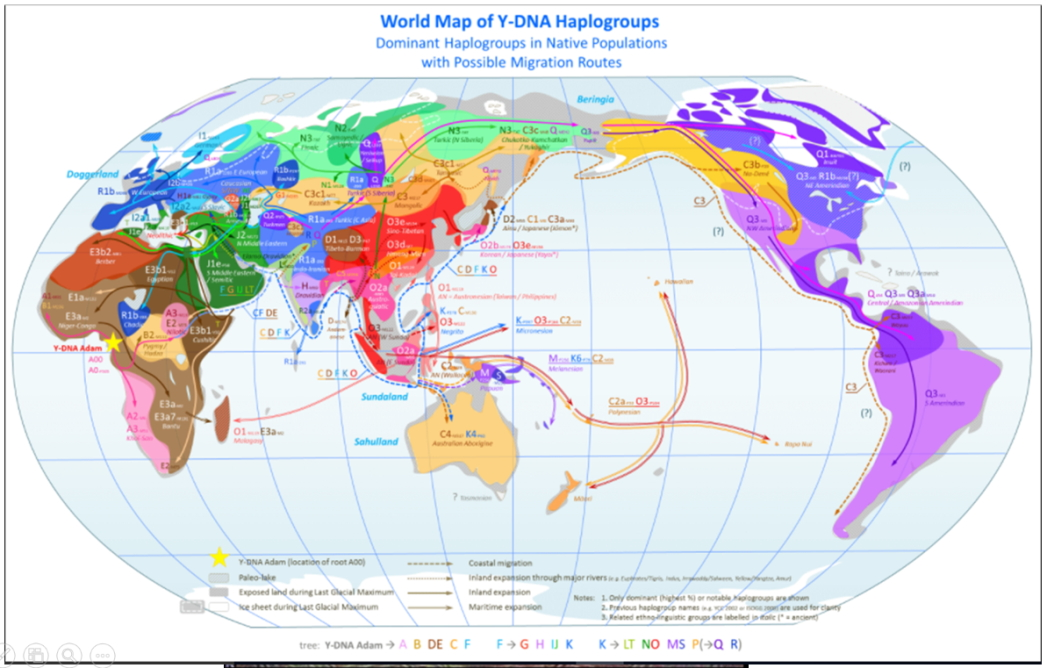
\includegraphics[scale=0.18]{images/8-12.jpg}
\caption{}\label{art8-fig12}
\end{figure}

The culture depicted in both Mahābhārata\index{Mahabharata@Mahābhārata} and Rāmāyaņa has Sanskrit language at its core and both epics allude to existence of Ṛgveda long before the events described in them. Thus, presence of Sanskrit language and Sanskrit language based culture can be shown to have existed, in abundance, within India during 6th millennium BCE (Mahābhārata) and 13th millennium BCE (Rāmāyaņa\index{Ramayana@Rāmāyaņa}) and is depicted in Figure 13.

\begin{figure}[!htbp]
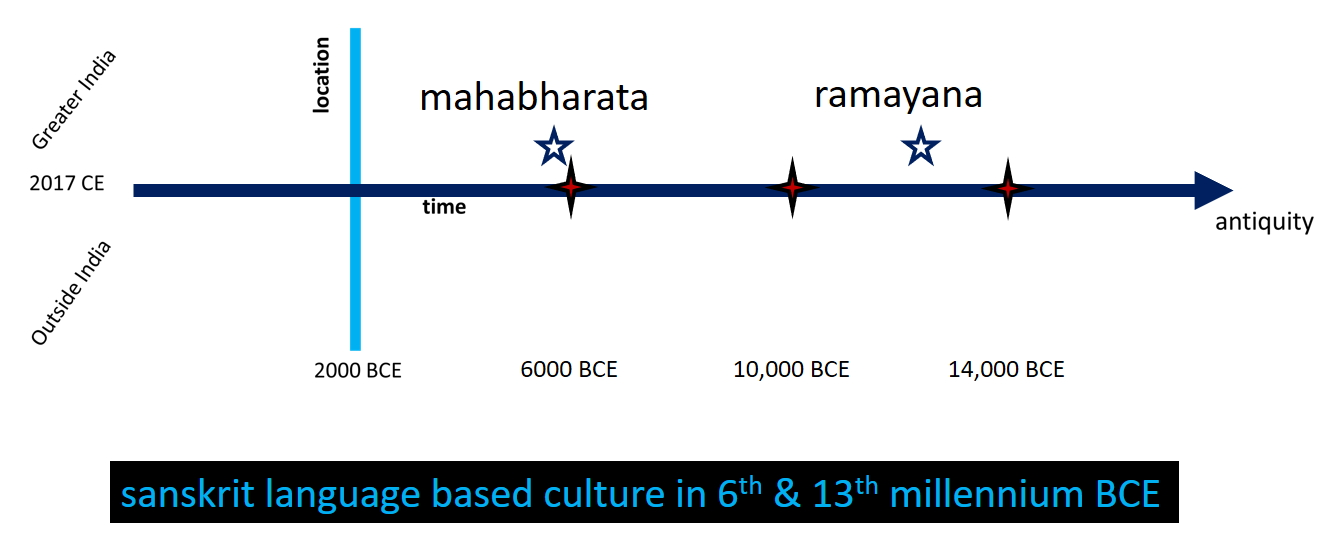
\includegraphics[scale=0.19]{images/8-13.jpg}
\caption{}\label{art8-fig13}
\end{figure}


\paragraph*{2.6.1.1 Tāmasic skepticism of astronomy evidence}

What shocks many a researcher of these astronomy studies are the timelines arrived at due to scientific testing of astronomy evidence\index{astronomy evidence} from these epics. A number of researchers who have learnt to produce their research to fit the existing paradigm for antiquity of human civilizations are flabbergasted by claims of such deep antiquity. This is all to be expected. All revolutionary discoveries have this effect of rousing sleepy researchers from their slumber. This should lead them to investigate and test these claims. Unfortunately, the reaction of many is emotional, and instead of focusing their efforts on comprehending these claims and then critiquing them – brutally and rationally, these researchers criticize these claims with any irrational means they can find at their disposal. The reasons for such ignorance could be many and may be a subject of separate research effort.

It would be useful for these researchers to realize that a typical measure of scientific success is the ability of a scientific theory to deliver novel predictions, which – if experimentally proved – might constitute an important advance for our scientific knowledge, in general, and an important advance for our knowledge of ancient Indian history, in this specific case.

A recurring and false accusation, from all and sundry, claims that these claims were arrived at based on one or two isolated astronomy observations. This is far from the truth. In fact, investigation of Mahābhārata astronomy evidence presented (Oak, 2011) is the first and only comprehensive investigation that considers all astronomy evidence of the Mahābhārata text and objectively tests it within the scientific framework. The second investigation (Oak, 2014) is also the first and only comprehensive investigation that considers all astronomy evidence of Vālmīki Rāmāyaņa text and objectively tests it within the scientific framework.

Another recurring objection refers to lack of any additional astronomy evidence that also points to such deep antiquity. This is again an unjustified and unfounded objection. The reality is enormous evidence is already being found and much new evidence is on its way, purely from the field of astronomy that leads to event horizon into further antiquity that already established by the timeline for the epics. Only by way of illustration, few events along the last 17,000-year long timeline are presented.


\paragraph*{2.6.1.2 Updates in Sūrya Siddhānta}

Sūrya Siddhānta\index{Surya Siddhanta@Sūrya Siddhānta} is an ancient Indian text. Like many Indian classical works, it is written in verse form and in Sanskrit language. The text covers cosmology, planetary motions, eclipses, conjunctions, star positions, rising/settings, mathematics, geography, instrumentation and model-making. It is not a conventional textbook. It is too succinct and somewhat cryptic for a rank beginner. It is rather meant as a concise aid to instruction for the experienced teacher. The texts like Sūrya Siddhānta have been highly revered books since ancient times and ancient Indian astronomers would be hesitant to make any substantial changes unless the mistake was glaring. The variables such as equation of the sun, latitudes, obliquity of the earth's axis will have only small changes over thousands of years and are likely to be left alone.

\vskip 3pt

Excellent work of Shri Anil Narayanan (2010, 2011) leads to identification of three specific updates to Sūrya Siddhānta. All the star longitudes in the Sūrya Siddhānta match with actual star longitudes of around 570 CE. Thus, there is the strong possibility that the last update to the longitudes were done at that time, plus or minus a hundred years.

\vskip 3pt

Chapter 8 of the Sūrya Siddhānta gives the latitudes and longitudes of several stars. Now while star latitudes change very slowly, longitudes change quickly due to precession, about 1 degree every 70 years. Narayanan (2010) made an intriguing discovery and further investigation with the help of computer simulation that involved stellar proper motions, ecliptic-obliquity variation, ecliptic node location variation and ecliptic sink variation for latitudinal data resulted in identification of another instance of update around 7300 BCE-7800 BCE.

\vskip 3pt

Narayanan (2011) found that when compared to the current value of the equation of the Sun, the value given in the Sūrya Siddhānta is quite off the mark. But as one goes back in time, the Sūrya Siddhānta value comes closer and closer to the actual equation of the Sun, and around 5300 BC, the error is less than 1 minute of arc. Thus, assuming the equation of the Sun was measured accurately by the ancient Indian astronomers, and the fact that the error in the Sūrya Siddhānta value drops to 1 minute of arc in 5300 BC, we can surmise that the Sūrya Siddhānta data for the equation of the Sun was last updated around 5300 BCE (5000 BCE – 5500 BCE).

Bhaty \& Oak (2017) identified another update event in Sūrya Siddhānta around 12000 BCE which is been corroborated not only by modern astronomy but also by corroborative evidence of Rāmāyaņa. These four updates in Sūrya Siddhānta are summarized, and superimposed on the chronology of the epics in Figure 14.

\begin{figure}[!htbp]
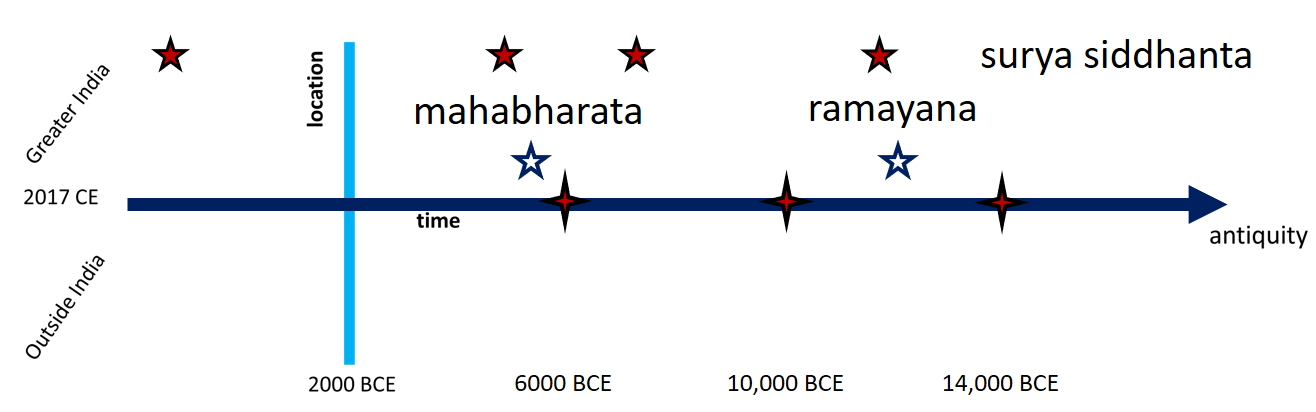
\includegraphics[scale=0.2]{images/8-14.jpg}
\caption{}\label{art8-fig14}
\end{figure}


\paragraph*{2.6.1.3 Update in Śatapatha Brāhmaņa}

This phenomenon of updates is not a sporadic phenomenon and rather a norm for all smṛti literature of India. Śatapatha Brāhmaņa\index{Satapatha Brahmana@Śatapatha Brāhmaņa} refer to rising of nakṣatra Kṛttikā\index{Krttika@Kṛttikā} in the true east direction while no other nakṣatra was rising true east when this update was recorded.

Numerous western Indologists have deliberately twisted this reference to claim recent timing (as late as 500 BCE) of this update. In a series of blog articles Oak (2014, nileshoak.wordpress.com) showed that not only the timing of this update, as first discovered by great astronomer late Shankar Balakrishan Dikshit, is indeed around 3000 BCE, but also the precision employed by the astronomers is within +-/ - 100 years. This means the timing of this update can-not be any time after 2900 BCE. This update is summarized along with other chronology markers in Figure 15.

\begin{figure}[!htbp]
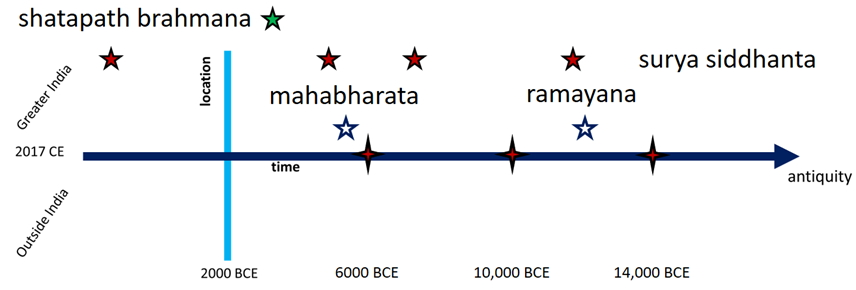
\includegraphics[scale=0.3]{images/8-15.jpg}
\caption{}\label{art8-fig15}
\end{figure}


\paragraph*{2.6.1.4 Ancient events mentioned in epics}

Finally, let’s consider a scenario where memory of an ancient event is preserved in the text. The Mahābhārata text preserves a memory of an ancient event that can be estimated to have occurred sometime in 15th millennium BCE, the famous reference to fall of Abhijit. Oak (2011) describes the objective testing of this astronomy observation that leads to a timing interval of 14600 BCE through 14900 BCE. Both epics refer to the incident of sage Viśwāmitra\index{Viswamitra@Viśwāmitra} creating Prati-sṛṣṭi by assigning first place to nakṣatra Śravaņa\index{Sravana@Śravaņa} and that this was the time of king Triṣańku\index{Trisanku@Triṣańku}. When these astronomy references are interpreted in the context of Rāmāyaņa timeline and fall of Abhijit, it naturally leads us to the timing of 13, 000 BCE. These events are summarized in Figure 16.

\begin{figure}[!htbp]
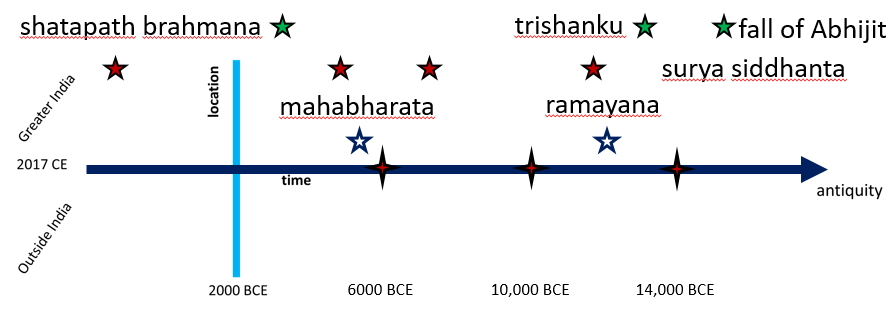
\includegraphics[scale=0.3]{images/8-16.jpg}
\caption{}\label{art8-fig16}
\end{figure}


\paragraph*{2.6.1.5 Why limit to only astronomy evidence}

It is not unusual to hear of another objection which takes the form of, “Why limit to only astronomy evidence?’. The very objection smacks of much ignorance of how scientific research works. No sensible researcher would advocate or insist on one specific discipline of science and related evidence as the only choice or even a preferred choice. The availability of evidence determines the discipline of science employed in exploring and testing such evidence. Thus, the question, ‘why limit to only astronomy’ evidence is redundant.

Having said that, there is much about the superiority of astronomy evidence, when it is indeed available, and fortunately, it can be exposed to severe objective tests. And while there are no guarantees in what any piece of evidence and its testing would reveal, astronomy evidence is the only evidence that can predict the chronology of ancient events precisely, down to the year, month and day. This also allows brutal, factual and objective criticism of claims that are due to result of astronomy evidence.

These claims, based on astronomy, evidence should be compared and challenged by evidence from other disciplines of science. This has been accomplished in the rest of this paper, as follows.

\newpage

\subsection*{2.6.2 Oceanography evidence\index{Oceanography evidence} for flooding \& destruction of Dwarka}

Oak (2011) tested more than 200 astronomy observations to arrive at 5561 BCE as the year of Mahābhārata war. Mahābhārata text refers to flooding and destruction of Dwarka\index{Dwarka}, 36 years after the war. Thus, the predicted year for flooding and destruction of Dwarka is 5525 BCE (36 years after 5561 BCE).

Since Dwarka was assumed to be situated on the west coast of India, the evidence for its flooding can be searched among the records of oceanography evidence. It is important to remember that a specific coastal location may have evidence for numerous floods, Tsunamis or earthquakes and thus such evidence is only useful if the claim for flooding and/or destruction is being made via evidence from other discipline(s) of science. Thus, the question we ought to ask is, “is there compelling evidence for flooding or sudden rise of sea levels at postulated location of ancient Dwarka, in the year 5525 BCE?”. The answer to that question is resounding ‘yes!’.

Enormous evidence exists that refers to sudden rise of sea levels, around the world, in 6th millennium BCE. Let’s look at some of the key evidence from around the world.

Blanchon et al (1995) presented evidence of sudden significant rise, termed by them as CRE (critical rise event) in the sea level of about 6.5 m (+/- 2.5 m) around 7600 BP (5600 BCE (+/- 140 years)) as far as Caribbean-Atlantic region. Ryan et al (1997) refer to abrupt drowning of Black Sea shelf due to inflow of Mediterranean water into the Black sea region during 7550 calendar years BP, which is about 5550 BCE. Ryan \& Pitman (1998) demonstrated the timing of the event of Black sea to be that of 5525 BCE. The calendar ages of relevant samples were 7500, 7580, 7510, 7510, 7470 calendar years with one sigma error of only 35 to 50 years, thus providing impressive corroboration for predicted year of 5525 BCE.

Before someone wonders what the significance of presenting these studies far from the west coast of India is, let me present two studies from the region of west coast of India. Zarins (1992) shows evidence of significant rise in the sea level of about 20 m within, in the Arabian Sea during 6th millennium BCE. The picture is worth thousand words and this is indeed true in this composite graph shown in Figure 17 (Zarins, 1992), based on seven independent studies, which should remove all remaining doubts. The X axis scale is the time scale with years read from the left (numbers at the top) in BCE until the scale reaches zero. Further right to the zero the scale continues in CE years. Bhonde et al (2011) have also shown a break during early Holocene (6th millennium BCE), on the west coast of India (Gujarat region), representing the low sea level stand.

\begin{figure}[!htbp]
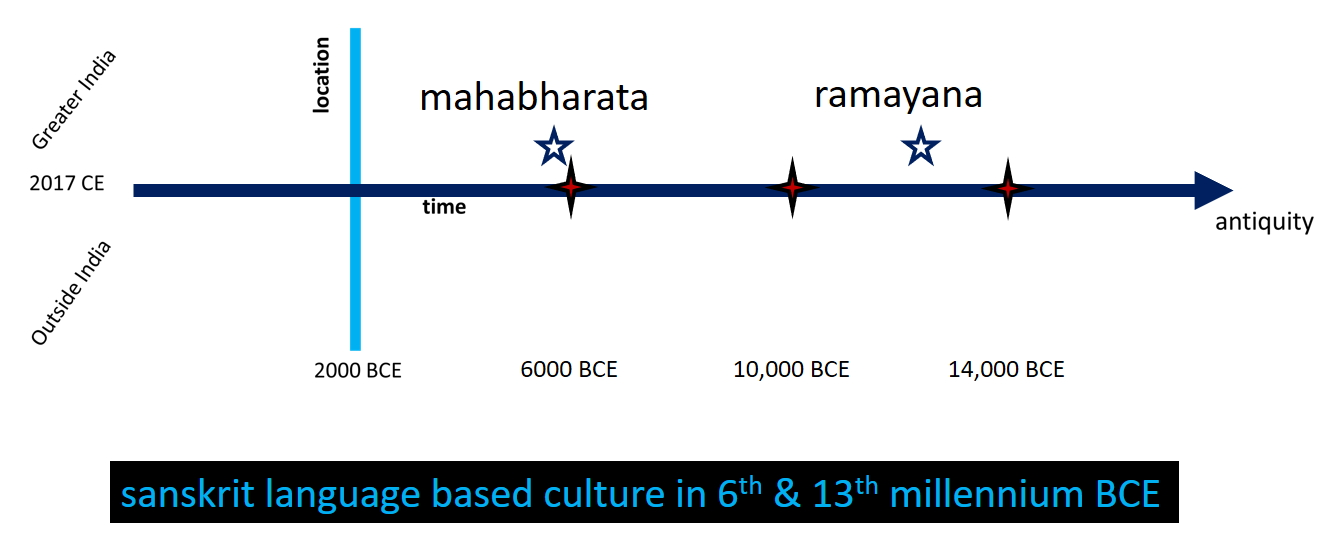
\includegraphics[scale=0.33]{images/8-17.jpg}
\caption{}\label{art8-fig17}
\end{figure}

In conclusion, oceanography evidence, around the world, including the relevant area of plausible location of Dwarka (Mūl Dwārakā, Gulf of Cambay) demonstrate significant evidence of sudden and catastrophic sea level rise during 6th millennium BCE and specifically for the timing of 5525 BCE. This is a strong corroborative evidence for the claim of flooding and destruction of Dwarka for the year 5525 BCE, a claim based on astronomy evidence internal to the Mahābhārata text after testing more than 200 astronomy observations.


\subsubsection*{2.6.3 Seismology evidence for flooding \& destruction of Dwarka}

While many of us have visited Dwarka\index{Dwarka} near Porbandar in Gujarat, India, very few of us know of a small place called ‘Mūl Dwārakā’ that is located south of Somanath. The current temple of Krishna in Dwarka is about 900 years old.

Let’s begin with the conjecture that the small town of ‘Mūl Dwarka (translated as ‘original Dwarka) is a proxy for the original Dwarka of Krishna as it points to the area of original Dwarka that is now underwater. The location of ‘Mūl Dwārakā’ is along the coast, in the modern state of Gujrat in western India as shown in Figure 18.

\begin{figure}[!htbp]
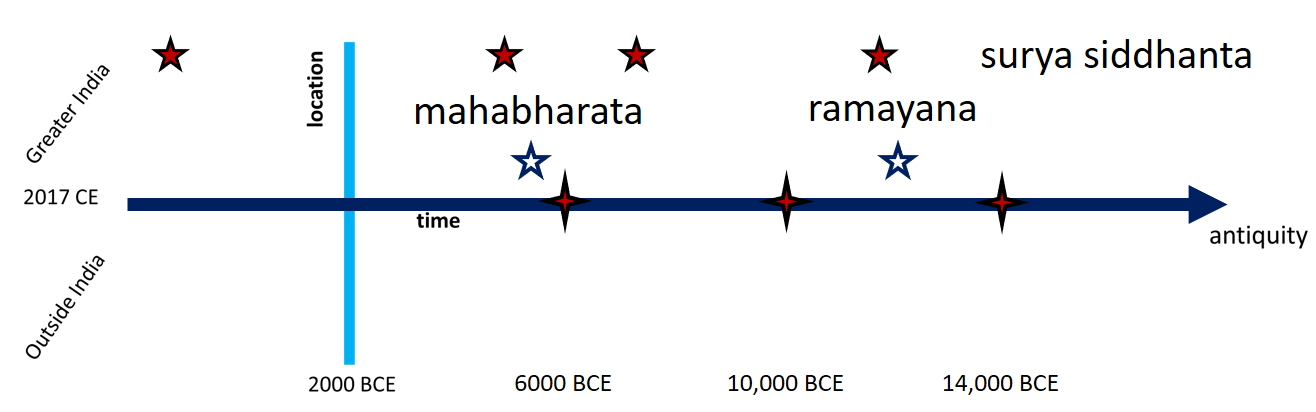
\includegraphics[scale=0.4]{images/8-18.jpg}
\caption{}\label{art8-fig18}
\end{figure}

The area is active seismic zone. Several earthquakes have affected this area for past few centuries, including the recent 8+ Richter scale earthquake on 26 January 2001 CE. O 16 January 1819 CE, an 8.3 magnitude earthquake affected this area.

It is critical to note that these earthquakes lead to lot of subsidence (land going down/sinking) and elevation at other places. This seismic activity leads to changes in the height of sea floors and not just land. These factors must be considered, along with sea level changes while researching ancient historical events. Various surveys, around the gulf of Cambay have picked up fault zones with elevation and depression of as much as 30 m. The gulf of Cambay was formed by a major rift.

Dr. Rajendran of National Center for Earth Science Studies, Trivenrum (now working at IISc, Bangalore) commissioned ‘paleo-seismic’ studies in this area. His excellent work led to identification and dating of ancient seismic events in this region. The major earthquakes events identified in this region belong to 7540 BP (+/- 130), 3983 BP (+/- 150) and 2780 BP (+/- 150). The evidence of 7540 BP, i.e. about 5540 BCE (+/-130 years) provides a corroborative event for the claim of flooding and destruction of Dwarka in 5525 BCE. Updated chronology scenario validated via various disciplines of science, for ancient Indian civilization is summarized in Figure 19.

\begin{figure}[!htbp]
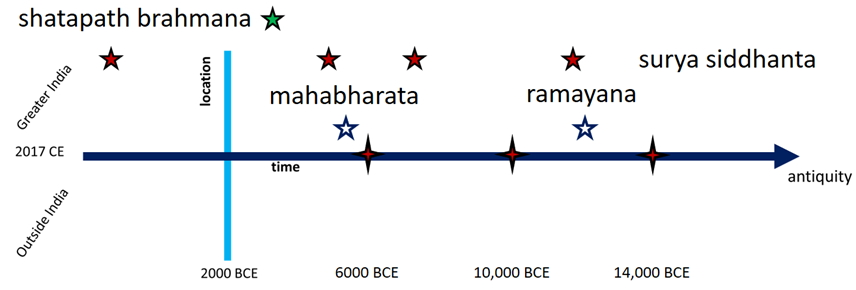
\includegraphics[scale=0.31]{images/8-19.jpg}
\caption{}\label{art8-fig19}
\end{figure}


\subsubsection*{2.6.4 River Sarasvati evidence: nightmare of AIT proponents}

Aryan invasion theory claims that Sanskrit or precursor to Sanskrit language did not exist in India prior to 2000 BCE and thus Ṛgveda or any Sanskrit based culture could not have existed in India, prior to 2000 BCE. No wonder, evidence of not only Mahābhārata and Rāmāyaņa but also Ṛgveda and presence of Sarasvati river\index{Sarasvati river} in India, prior to 2000 BCE, send shivers through the spine of AIT proponents and their heart palpitations increase.

In this section, impressive corroboration of descriptions of river Sarasvati from Mahābhārata\index{Mahabharata@Mahābhārata}, Rāmāyaņa\index{Ramayana@Rāmāyaņa} and Ṛgveda\index{Rgveda@Ṛgveda} with hydrology, geology, geophysics, genealogy evidence which in turn is corroboration of absolute chronology of epics and relative chronology of Ṛgveda is presented.

Figure 20 (Hector, 2017) shows broad paleochannel\index{paleochannel} of river Sarasvati in the middle (Ghaggar-Hakra). North-west corner shows current path of river Satluj (Shutudri) and while eastern portion shows current path of river Yamuna. Multiple paleo-courses of river Shutudri could be seen between current path of river Shutudri and paleochannel of extinct river Sarasvati. Paleo-courses of river Yamuna could also be seen between current path of river Yamuna and paleochannel of river Sarasvati.

\begin{figure}[!htbp]
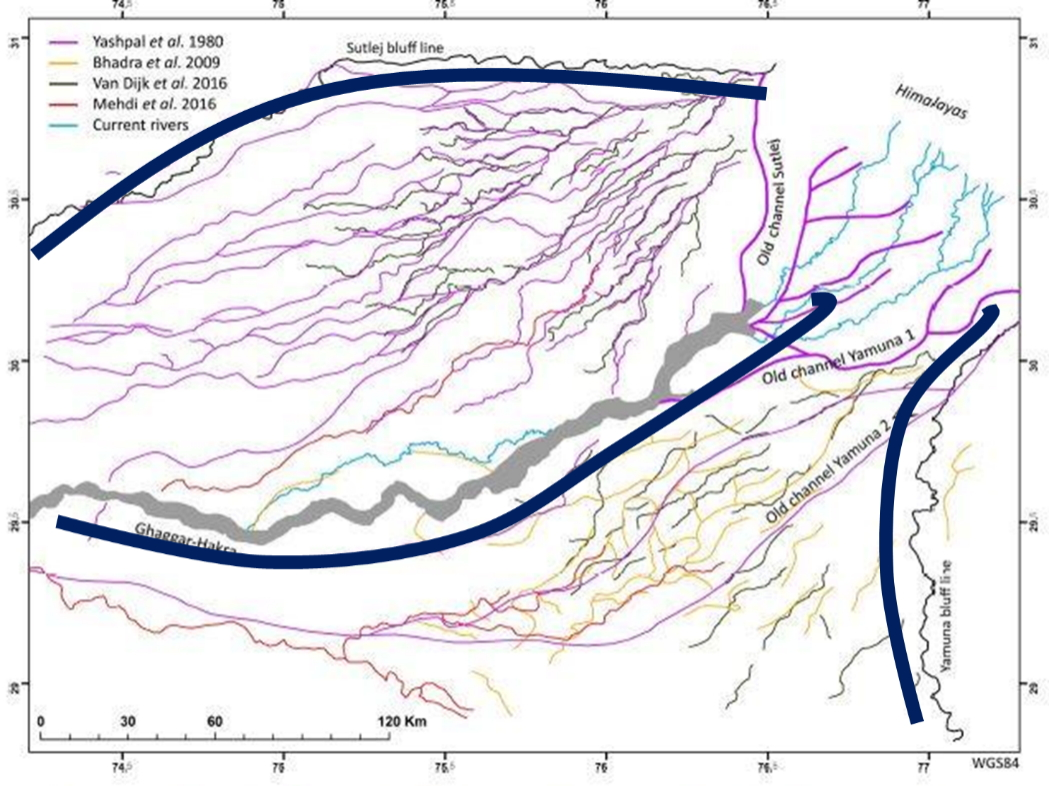
\includegraphics[scale=0.25]{images/8-20.jpg}
\caption{}\label{art8-fig20}
\end{figure}


\paragraph*{2.6.4.1 River Sarasvati: evidence from Mahābhārata \& Rāmāyaņa}

Oak (2011) has summarized descriptions of river Sarasvati from the Mahābhārata text. The river is described as flowing with plenty water in many places. On the other hand, the river is described as disappeared under the sand at many other places. The river had numerous holy places on its bank and Balarāma did pilgrimage of river Sarasvati while Mahābhārata war\index{Mahabharata war@Mahābhārata war} was taking place.

Oak (2014) has enumerated descriptions of river Sarasvati from the Vālmīki Rāmāyaņa text. The river is no longer the grand river of Ṛgveda; river Yamuna has already separated from river Sarasvati and has merged with river Ganga. River Shutudri has already turned sharp west and thus no longer feeding its waters into river Sarasvati.


\paragraph*{2.6.4.2 River Sarasvati: hydrology, climatology and geology/\break geophysics evidence}

Significant hydrology and geology research has taken place in the context of river Sarasvati and its paleo-tributaries. Clift and his research team (2012) showed that river Yamuna separated from river Sarasvati as early as 50,000 BCE and no later than 9000 BCE. Francfort and his research team (1992) reached the same conclusion more than 30 years ago when they asserted that the paleo-courses of river Sarasvati were dry from early Holocene or even earlier. Danino\index{Danino, Michel} (2010) refers to numerous studies that indicate intensification of monsoon in India’s northwest sometime after 9000 BCE that went back to current levels around 4000 BCE. His work also sites other studies that asset the complete drying up of river Sarasvati by about ~2000 BCE.

This evidence from various disciplines of science – hydrology, climatology, geology and geophysics\index{geophysics} corroborates well with textual descriptions of the Mahābhārata and Vālmīki Rāmāyaņa\index{Ramayana@Rāmāyaņa} text and with chronology of these epics arrived via internal astronomy evidence. This triangulation of scientific evidence with textual and chronology evidence is represented in Figure 21 and the summary of their corroboration is presented in Figure 22.

\newpage

\begin{figure}[!htbp]
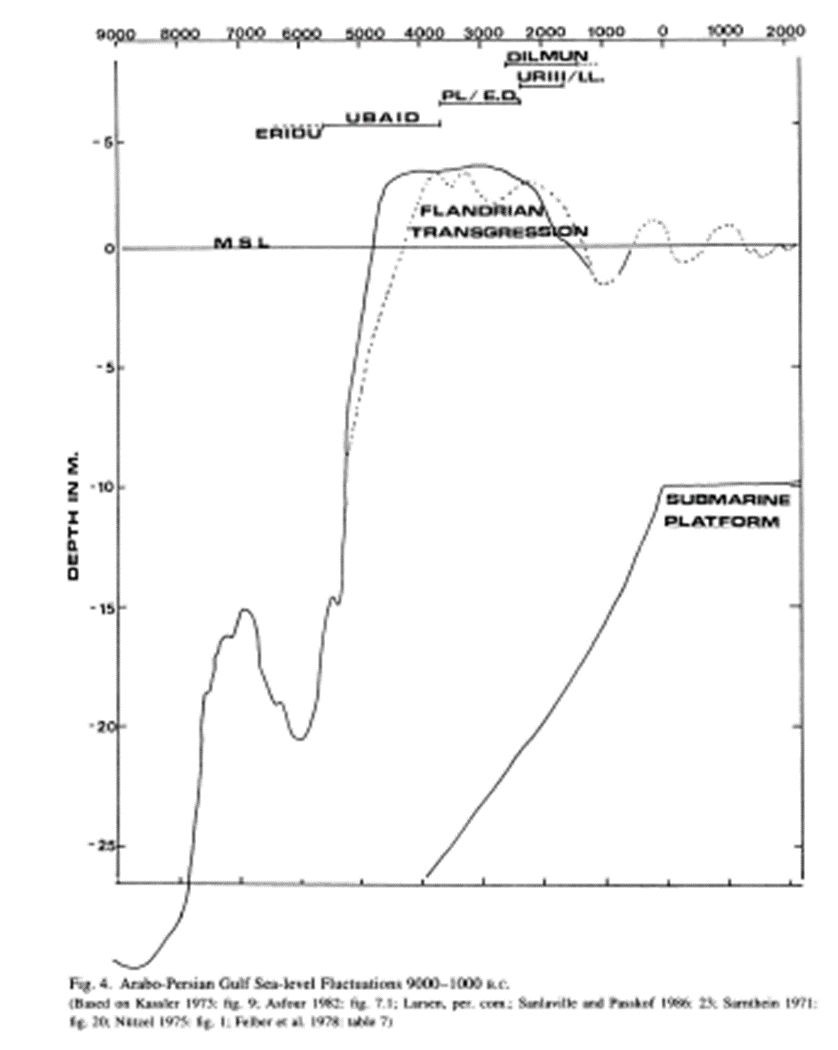
\includegraphics[scale=0.2]{images/8-21.jpg}
\caption{}\label{art8-fig21}
\end{figure}


\begin{figure}[!htbp]
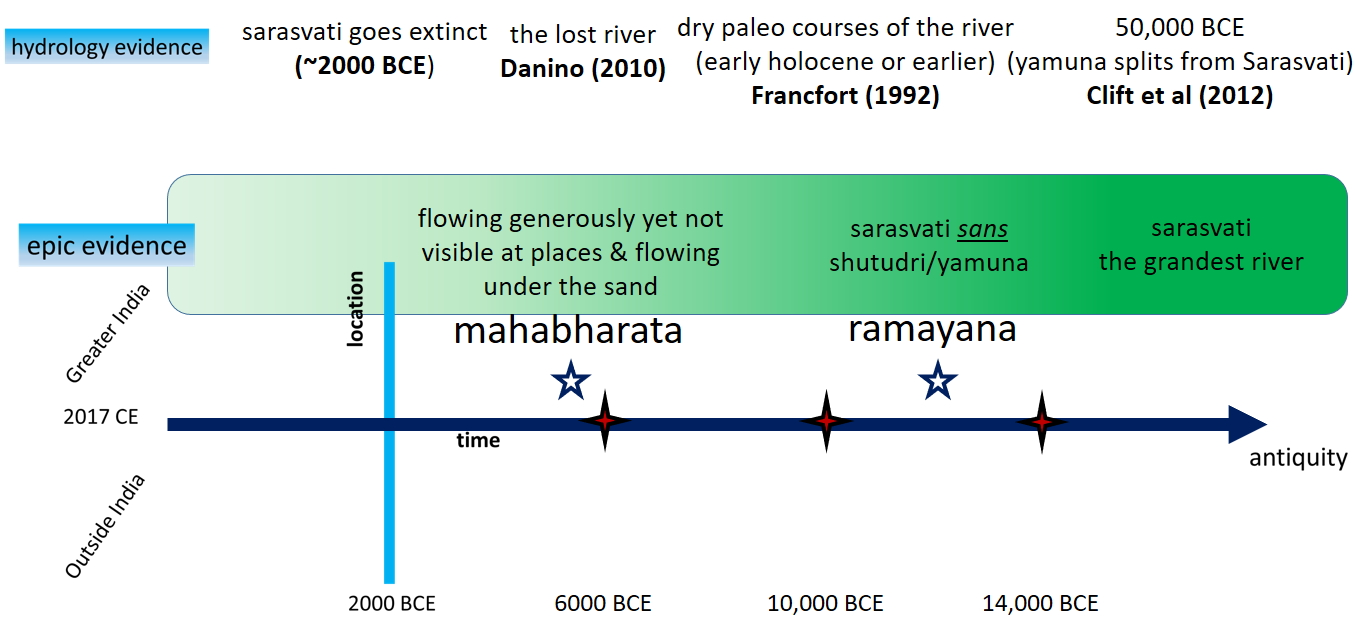
\includegraphics[scale=0.2]{images/8-22.jpg}
\caption{}\label{art8-fig22}
\end{figure}


\paragraph*{2.6.4.3 River Sarasvati: Ṛgveda – Relative Chronology \& Hydrology Evidence}

Ṛgveda is the oldest extant text of humanity, it has 10 maņḍala-s, and it is indeed difficult to determine when its earliest portions were composed. The text was not inspired/conceived/composed at one time and Talageri (2000) did an impressive research to determine the relative chronology of its 10 maņḍala-s by employing multiple internal elements of Ṛgveda text. Per this chronology, Maņḍala-s 6,3, 7 are the oldest maņḍala-s, followed by 4 and 2, respectively. Then come Maņḍala-s 5, 8 and 9. Maņḍala 10 is the youngest maņḍala and there is a significant gap, of unknown duration, between maņḍala 9, last of the previous maņḍala-s and maņḍala 10. Sūkta-s of maņḍala one can be divided into three broad categories that align with early, middle and the last maņḍala-s of Ṛgveda.

What is fascinating is to note that all the references to grand Sarasvati, the biggest river among the rivers, the river that originates into the mountains and that reaches to the sea and more, occur in the earliest maņḍalas of Ṛgveda (6:61:2, 8, 10, 3:23:8, 7:95.1-2, 2:41.16). On the other hand, by the time we read the descriptions of rivers in the last maņḍala (maņḍala 10) of Ṛgveda, Sarasvati is no longer the grandest river, although it is still flowing and revered, but now it appears, that river Sindhu seems to have occupied that status (10.75.5-6).

Recall that descriptions of river Sarasvati from the epics have indeed drawn this picture of river Sarasvati that matches with not only astronomy evidence based chronology of the epics but also hydrology, geology and climatology evidence based chronology for the state of river Sarasvati.

\begin{figure}[!htbp]
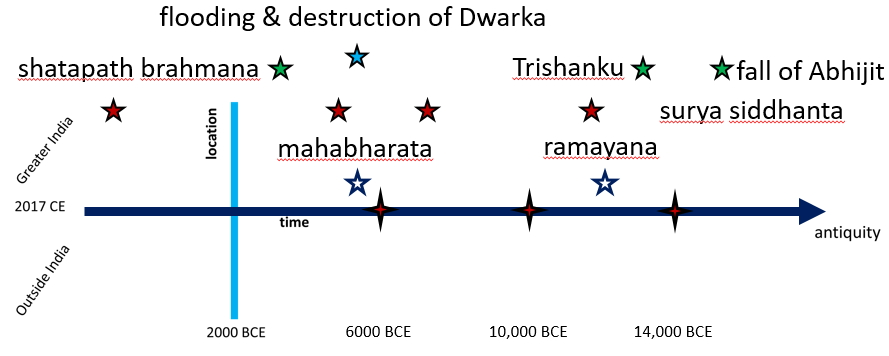
\includegraphics[scale=0.21]{images/8-23.jpg}
\caption{}\label{art8-fig23}
\end{figure}


\paragraph*{2.6.4.4 River Sarasvati: Ṛgveda, Rāmāyaņa \& Mahābhārata – Genealogy evidence}

A question may be raised, “This is all impressive; however, what could be our rational for aligning oldest maņḍala-s of Ṛgveda to a time earlier to Rāmāyaņa, middle maņḍala-s with the Rāmāyaņa time and the last maņḍala (maņḍala 10) with the Mahābhārata time. To answer this question, we will have look at genealogy evidence of Ṛgveda.

The oldest maņḍala-s of Ṛgveda (6.3. 7) are predominantly composed by sages of Vasishtha and Vishwamitra lineages who were most active prior to and during Rāmāyaņa times. The 10th and last maņḍala of Ṛgveda contains sūktas that mention Rama, Veņa and Pŗthu of Ikṣvāku lineage (10:93) and Śantanu and Devapi of Kuru lineage (10.93). King Śantanu was father of Bhīṣma and one may wonder how this information became part of the Ṛgveda. The answer is rather easy. Mahābhārata text tells us that Maharṣi VedaVyāsa did edit Vedas (Mahābhārata text critical edition: Adi 57:72-75) and thus we can infer that the last (10th) Maņḍala was edited during Mahābhārata times. This is our justification for aligning 10th maņḍala of Ṛgveda with the period of Mahābhārata.

Absolute chronologies of Rāmāyaņa, Mahābhārata corroborate exceedingly well with hydrology evidence of river Sarasvati, relative chronology of Ṛgveda Maņḍalas and with historical personalities mentioned in Ṛgveda. Thus, chronology proposal of 6th millennium BCE for Mahābhārata and 13th millennium BCE for Rāmāyaņa corroborate well with relative chronology of Ṛgveda, historical personalities of Ṛgveda,\break Rāmāyaņa \& Mahābhārata and hydrology evidence of river Sarasvati. These researches also assert chronology of Ṛgveda to be prior to 13th millennium BCE and timing of 6th millennium BCE for the final editing of Ṛgveda. These are summarized in Figure 24.

\begin{figure}[!htbp]
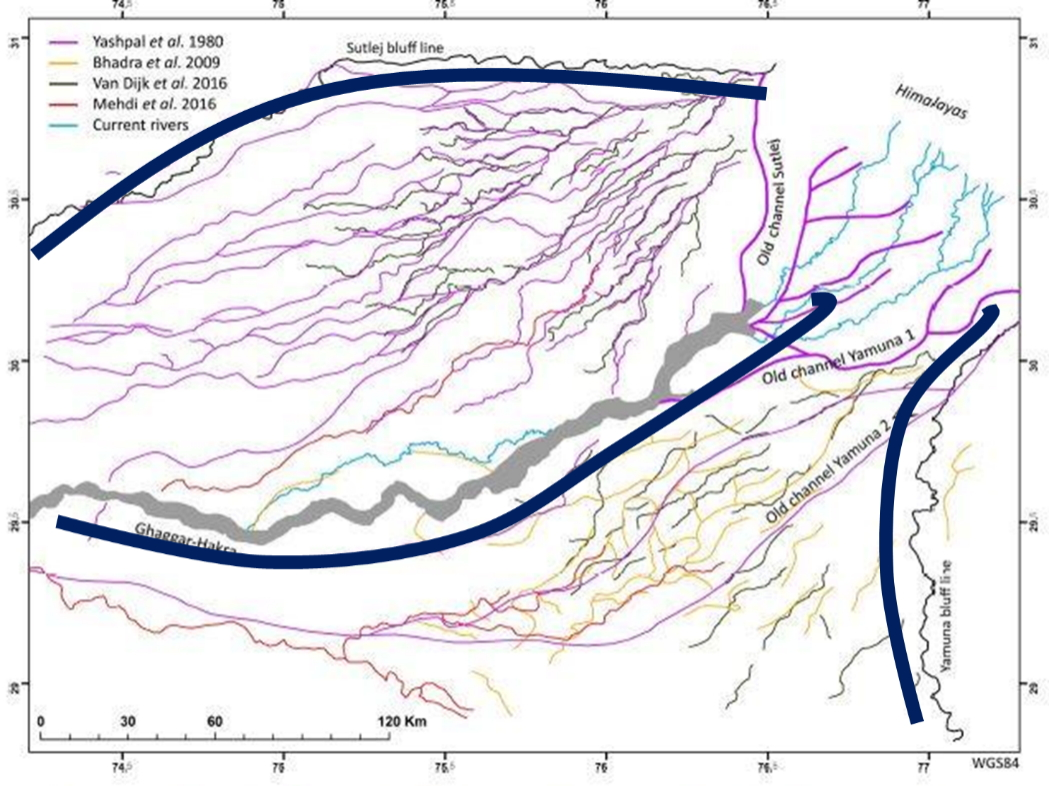
\includegraphics[scale=0.205]{images/8-24.jpg}
\caption{}\label{art8-fig24}
\end{figure}



\section*{Conclusions}

No evidence for ‘Aryan’ inside or outside India, prior to formulation of AIT in 18th century CE is found. Sanskrit language and Sanskrit language based culture existed in India that can be validated scientific evidence with high degree of testability. Such evidence pours in from multiple branches of science – astronomy, hydrology, climatology, geology, geophysics, genealogies of kings and sages of Ṛgveda\index{Rgveda@Ṛgveda}. Linguistics claims of AIT were not only falsified via linguistics by work of Shri Talageri but also his work decisively showed that the language flow, if it did occur, occurred from India to outside India. Archaeology evidence showed continuous civilization in India for at least last 9000 years and genetics evidence shows out of India matrilineal and patrilineal gene flow over last 40,000+ years.

The word “ārya” was an honorific word meaning righteous and noble, very much of Indian and Sanskrit origin and the word was found nowhere outside greater India prior to direct contact of Europeans with India. India had Sanskrit language based continuous civilization for more than 17,000 years and its key chronology landmarks can be traced with the help of objectively testable evidence with the logic of scientific method.

Aryan invasion theory\index{Aryan invasion theory} or its new incarnation – Aryan migration theory\index{Aryan migration theory}, is already being falsified. However, there is need to educate Indian population in a language they can comprehend and communicate to others.


\section*{Bibliography}

\begin{thebibliography}{99}
\bibitem{008-key01} Bhaty, Rupa \& Oak, Nilesh (2018). “Ancient Updates to Surya-Siddhanta” 9th Coffee-break conference, Science and technology in Premodern Asia, Oxford University, UK.

 \bibitem{008-key02} Bhonde, U et al (2011) “Discontinuity surfaces and event stratigraphy of Okha Shell Limestone Member: Implications for Holocene sea level changes, western India.” J. Earth Syst. Sci. 120, No 4, Pp. 723-734.

 \bibitem{008-key03} Blanchon, Paul et al (1995) “Reef drowning during the last deglaciation: Evidence for catastrophic sea-level rise and ice-sheet collapse”. Geology. v.23, 1, 4-8.

 \bibitem{008-key04} Bonhomme, F (2007) “Species-wide distribution of highly polymorphic minisatellite markers suggest past and present genetic exchanges among house mouse subspecies.” Genome Biology, 8: R80.

 \bibitem{008-key05} Clift, Peter et al (2012), \textit{”U-Pb zircon dating evidence for a Pleistocene Sarasvati river and capture of the Yamuna River”}. Geology.

 \bibitem{008-key06} Danino, Michel (2010) \textit{The Lost River: On the Trails of Sarasvati.} Penguin.

 \bibitem{008-key07} Francfort, Henri-Paul (1992) \textit{“Evidence for Harappan irrigation system in Haryana and Rajasthan”}. Eastern Anthropologist 45:Pp. 87-109.

 \bibitem{008-key08} Hector, Orengo (2017) “Large-Scale, Multi-Temporal Remote Sensing of Palaeo-River Networks: A Case Study from Northwest India and its Implications for the Indus Civilisation”. Remote Sens., 9, 735; doi:10.3390/rs9070735.

 \bibitem{008-key09} Lal, B. B. (2009) \textit{How Deep Are the Roots of Indian Civilization?: Archaeology Answers.} Aryan Books India.

 \bibitem{008-key10} Lal, B. B. (2002) \textit{The Saraswati Flows on the Continuity of Indian Culture.} Aryan books International, India.

 \bibitem{008-key11} Metspalu et al (2004) “Most of the extant mtDNA boundaries in South and Southwest Asia were likely shaped during the initial settlement of Eurasia by anatomically modern humans.” BMC Genetics 5:26.

 \bibitem{008-key12} Narayanan, Anil (2010) “Dating the Sūrya-Siddhānta using computational simulation of proper motions and ecliptic variations”. IJHS, 45:4, 455-476.

 \bibitem{008-key13} Narayanan, Anil (2011) “The pulsating Indian Epicycle of the Sun”, IJHS, 46.3, 411-425.

 \bibitem{008-key14} Oak, Nilesh (2011) \textit{When did the Mahābhārata war Happen? The Mystery of Arundhati.} Danphe Inc., USA.

 \bibitem{008-key15} Oak, Nilesh (2014a) \textit{The Historic Rama: The Indian civilization at the end of Pleistocene.} CreateSpace Independent Publishing, USA.

 \bibitem{008-key16} Ryan, William et al (1997) “An abrupt drowning of the Black Sea Shelf.” Marine Geology, 138, 119-126.

 \bibitem{008-key17} Ryan \& Pitman (1998) \textit{Noah’s Flood: The New Scientific Discoveries About The Event That Changed History.} Simon \& Schuster.

 \bibitem{008-key18} Shastry, Shiv (2017a) “Migrations, Yes; But ‘Aryan’ Migrations? Not Really”. Swarajya Magazine, 25 June 2017, India.
 
 \bibitem{008-key19} Shastry, Shiv (2017b) “Aryans And Dravidians: An Invention of Racist Nineteenth Century Scholars.” Swarajya Magazine, 25 June 2017, India.

 \bibitem{008-key20} Talageri, Shrikant (1993) \textit{The Aryan Invasion Theory and Indian Nationalism.} New Delhi: Voice of India.

 \bibitem{008-key21} Talageri, Shrikant (2000) \textit{The Ṛgveda – A Historical Analysis.} New Delhi: Aditya Prakashan.

 \bibitem{008-key22} Talageri, Shrikant (2008) \textit{The Ṛgveda and the Avesta – The Final Evidence.} New Delhi. Aditya Prakashan.
 
 \bibitem{008-key23} Zarins, Juris (1992) “The Early Settlement of Southern Mesopotamia: A Review of Recent Historical, Geological and Archaeological Research.” Journal of the American Oriental Society, Vol 112, No. 1, 55-77.

 \bibitem{008-key24} Wikipedia. “Map of migration of Y chromosome bearing humans according to the recent African origin of modern human theory.” \url{https://en.wikipedia.org/wiki/Human_Y-chromosome_DNA_haplogroup}. Accessed on 1 September 2017.

 \bibitem{008-key25} Wikipedia. “World map of Y-DNA Haplogroups.” \url{https://en.wikipedia.org/wiki/Human_Y-chromosome_DNA_haplogroup#/media/File:World_Map_of_Y-DNA_Haplogroups.png}. Accessed on 1 September 2017.

 \bibitem{008-key26} Oak, Nilesh. Blog article at \url{https://nileshoak.wordpress.com}. \url{https://nileshoak.wordpress.com/2014/02/13/nakshatra-krittka-rising-due-east-part-1/}. Accessed on 1 September 2019.

 \bibitem{008-key27} Oak, Nilesh. Blog article at \url{ https://nileshoak.wordpress.com}. \url{https://nileshoak.wordpress.com/2014/02/13/nakshatra-krittika-rising-due-east-part-2/}. Accessed on 1 September 2019.

 \bibitem{008-key28} Oak, Nilesh. Blog article at \url{https://nileshoak.wordpress.com}. \url{https://nileshoak.wordpress.com/2014/02/15/nakshatra-krittika-rising-due-east-part-3/}. Accessed on 1 September 2019.

 \bibitem{008-key29} Oak, Nilesh. Blog article at \url{https://nileshoak.wordpress.com}. \url{https://nileshoak.wordpress.com/2014/02/17/nakshatra-krittika-rising-due-east-part-4/}. Accessed on 1 September 2019.

 \bibitem{008-key30} Oak, Nilesh. Blog article at \url{https://nileshoak.wordpress.com}. \url{https://nileshoak.wordpress.com/2015/06/03/original-dwarka-earthquake-records/}. Accessed on 1 September 2019.

 \bibitem{008-key31} Badrinaryan, B. “Gulf of Cambay – Cradle of Ancient civilization (First published 1 February 2006). \url{https://grahamhancock.com/badrinaryanb1/}. Accessed on 1 September 2019.

 \end{thebibliography}

